\section{Software Update Platform}

Software Update Platform is responsible for performing updates on multiple devices and monitoring
installed applications. Developers prepare \emph{.deb} packages with applications and add them to
repository. When connection with device is established and information about update is written in
database, platform will perform software update on that device.


\subsection{Architecture}

Software Update Platform consists of two main parts:
\begin{itemize}
  \item client application installed on mobile device,
  \item server.
\end{itemize}

\begin{figure}[htbp]
  \centering
    \scalebox{0.9}{
      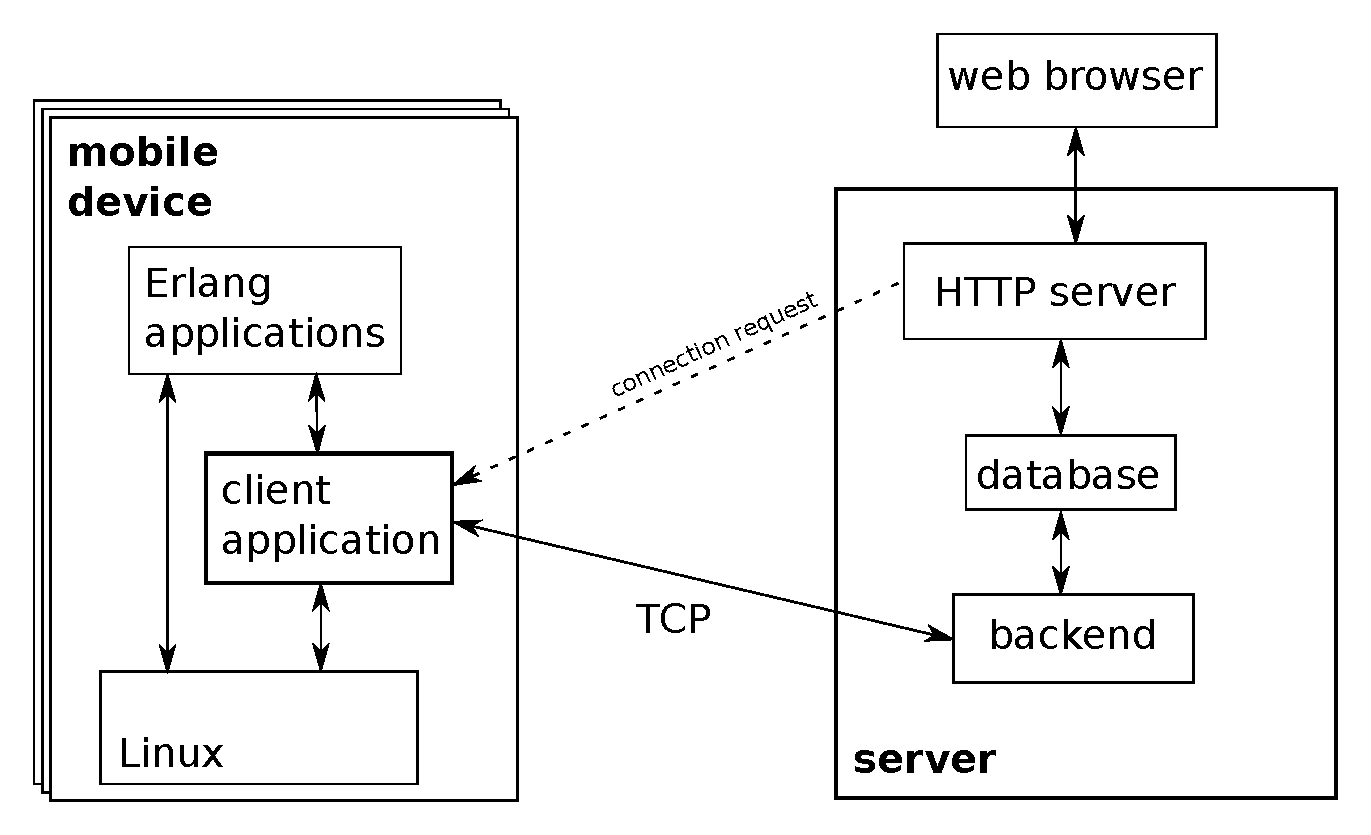
\includegraphics[width=\textwidth]{graphics/architecture.pdf}
    }
    \caption{Architecture overview}
\end{figure}

\subsubsection*{Client application}

We assume that client application is running on Erlang VM installed on some Linux distribution and
\emph{apt} is available. Client application connects with server and perform given operations.


\subsubsection*{Server}

Server consists of 3 components:
\begin{itemize}
  \item HTTP server
  \item database
  \item backend
\end{itemize}


\subsubsection*{HTTP server}

Mochiweb -- our web server of choice is responsible for following tasks. It manages user interaction
through web interface (serves content, performs user requests) and it is repository for \emph{.deb}
packages.


\subsubsection*{Database}

Mnesia database stores information about:
\begin{itemize}
  \item device and installed applications on it,
  \item jobs (e.g.\ update) for device.
\end{itemize}

\noindent Database is connector beetwen web interface and backend. It stores user requests -- jobs to perform
on device.


\subsubsection*{Backend}

Backend is the core of platform. It is Erlang application responsible for whole automatic device
management. Every new device in platform connected with backend is stored in database.
From now on backend can monitor state of that device and performs operations on it.

\subsubsection{Device-server session}

\begin{figure}[htbp]
  \centering
    \scalebox{0.9}{
      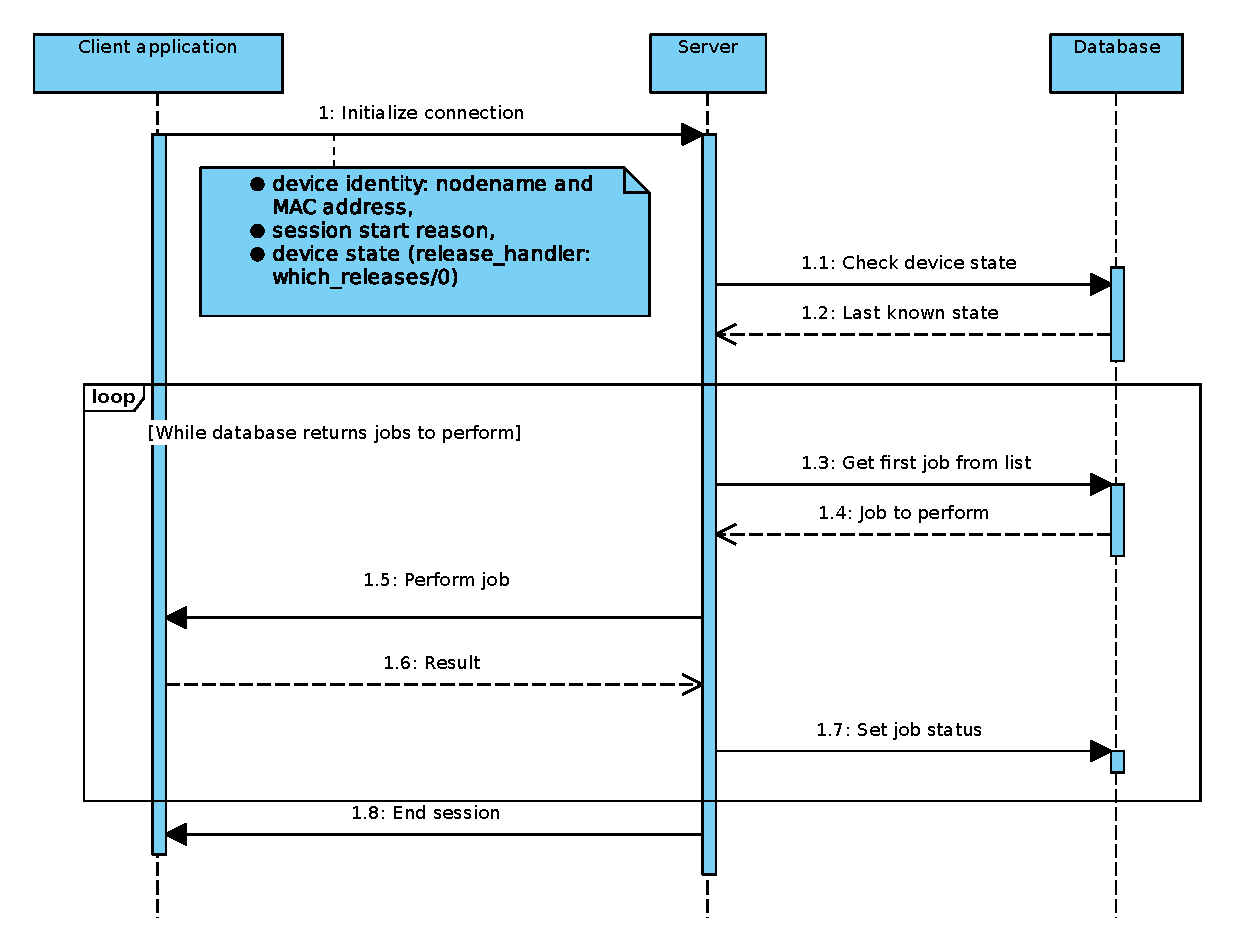
\includegraphics[width=\textwidth]{graphics/session.pdf}
    }
    \caption{Session communication diagram}
\end{figure}

Firstly device initializes connection which carries following data:
\begin{itemize}
  \item device identity: nodename and MAC address,
  \item session start reason,
  \item device states.
\end{itemize}
These pieces of information are used to unambiguously identify the device.
After connection is established, server checks device state in database.
If there are any enqueued jobs, they are sent to device.
The device returns result of performed job. This status is written to database.

\subsubsection{On-device upgrade logic}

Updating software consists of two jobs:
\begin{itemize}
  \item upgrade
  \item check release
\end{itemize}

Upgrade immediately returns with status \verb|ok|. It stops periodic connection requests, closes session and uses \emph{apt} to perform upgrade. It waits for \emph{apt} to finish and checks its result. Then it restores periodic connection requests.

Check release reads value returned from \emph{apt} and notifies server about changes in next session.

\subsection{Functionality}

\begin{itemize}
  \item General description of the Web interface

Web interface provides simple way to manage groups of devices. User can:
\begin{itemize}
  \item check last known state of device: IP, version of release, installed application
  \item assign device to one or more categories
  \item schedule jobs for device
\end{itemize}

\begin{figure}[htbp]
  \centering
    \scalebox{0.9}{
      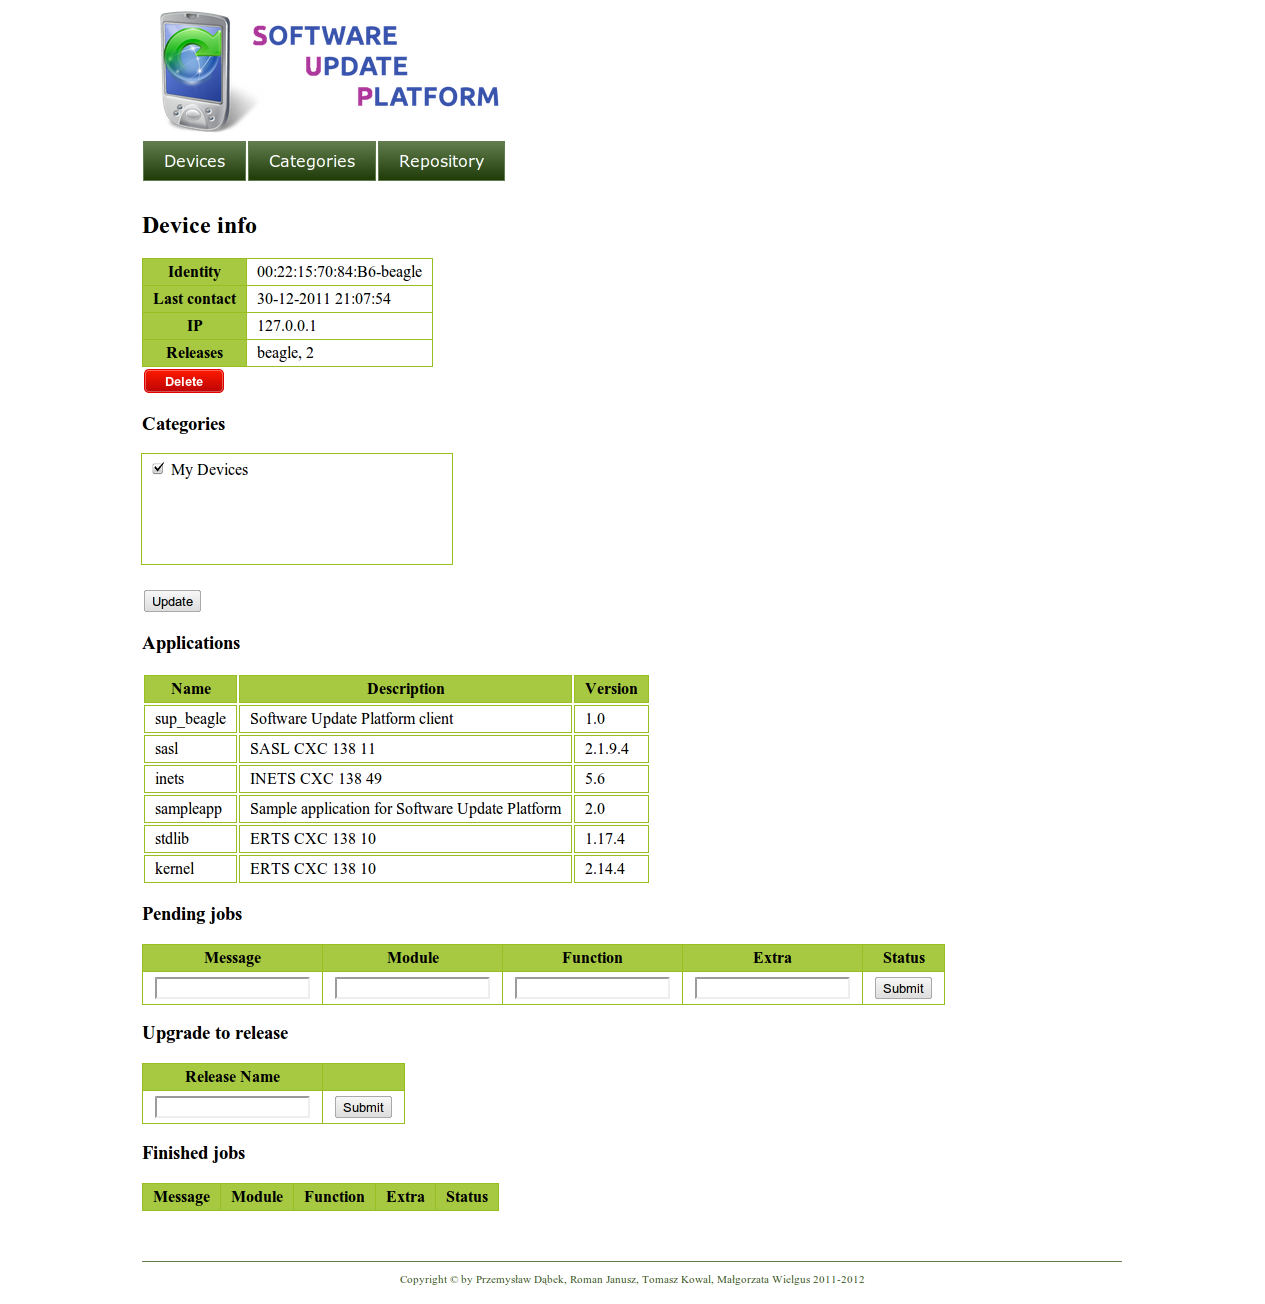
\includegraphics[width=\textwidth]{graphics/device.png}
    }
    \caption{Device view}
\end{figure}

\begin{figure}[htbp]
  \centering
    \scalebox{0.9}{
      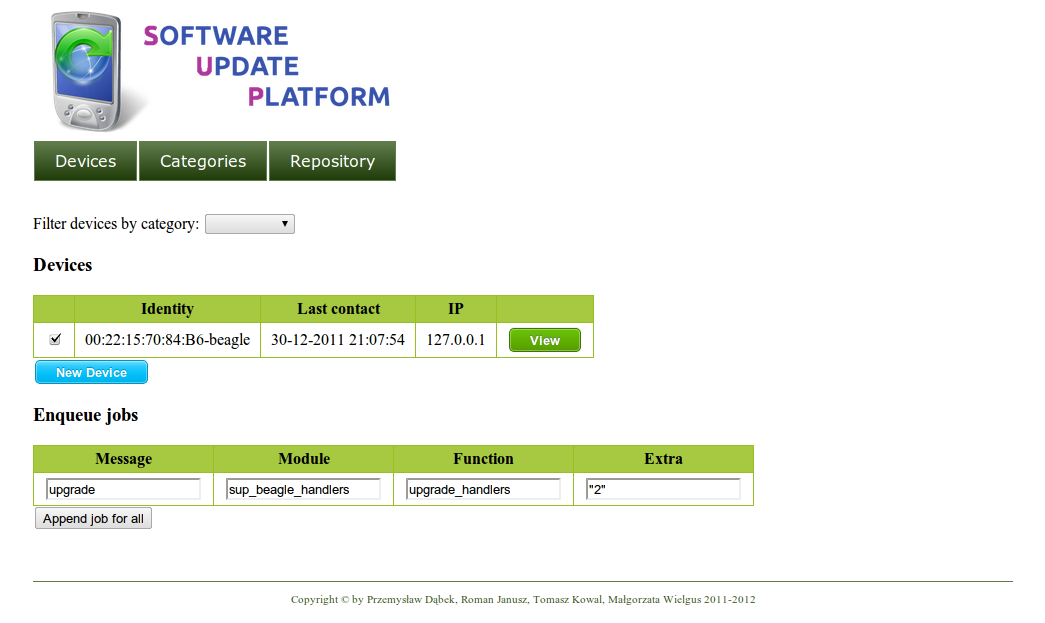
\includegraphics[width=\textwidth]{graphics/devices.png}
    }
    \caption{Device view}
\end{figure}

There is also special page for repository where user can upload previously prepared packages.

\begin{figure}[htbp]
  \centering
    \scalebox{0.9}{
      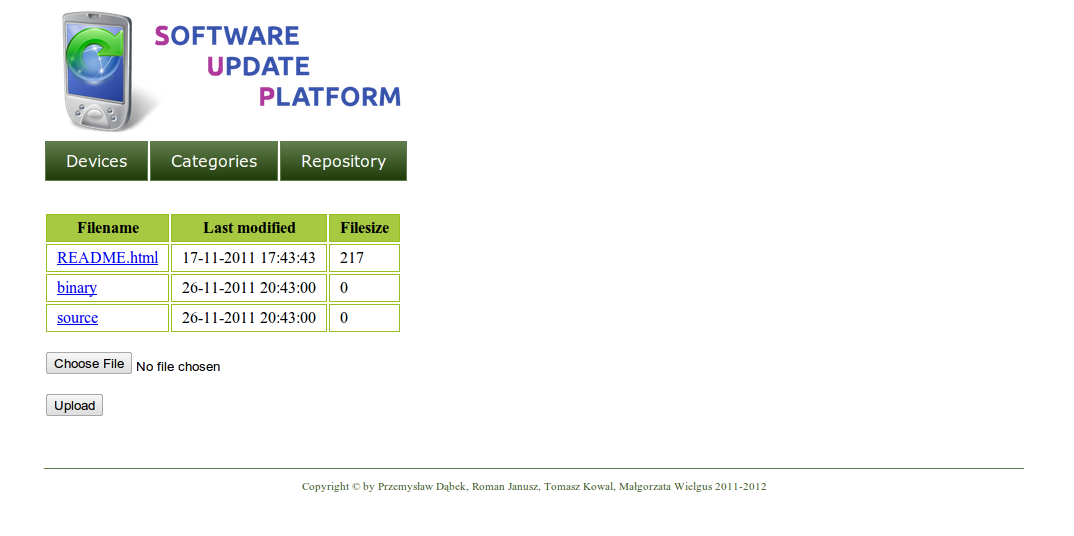
\includegraphics[width=\textwidth]{graphics/repository.png}
    }
    \caption{Repository view}
\end{figure}

    \item\label{devmodel} Development model for application, debian packaging utilities

Software Update Platform proposes a model and provides some tools for development of Erlang software installed
on the target systems. The main assumption is that the developer uses a tool called {\tt rebar} for managing Erlang software (see \cite{rebar} for more information).
{\tt rebar} is a script providing functionality for Erlang similar to what {\tt maven} provides for Java development.
This includes automatic generation of stubs for Erlang applications, build, {\tt .appup} file
generation, creation of complete, self-contained Erlang nodes (with a runtime), documentation etc.
Generated Erlang nodes are used as a basis for {\tt .deb} packages generation. This is implemented by a set of
scripts provided by the Software Update Platform itself.

\end{itemize}

